\documentclass[11pt]{article}

    \usepackage{listings}
    \usepackage{fancyhdr}
    \usepackage[margin=.8in]{geometry}
    \usepackage{amsmath}
    \usepackage{enumitem}
    \usepackage{hyperref}
    \usepackage{tikz}
    \usetikzlibrary{arrows}
    \tikzset{
        treenode/.style = {align=center, inner sep=0pt, text centered,
            font=\sffamily},
        arn_n/.style = {treenode, circle, black, font=\sffamily\bfseries, draw=black,
            fill=white, text width=1.5em},
        arn_r/.style = {treenode, circle, red, draw=red, 
            text width=1.5em, very thick},
        arn_x/.style = {treenode, rectangle, draw=black,
            minimum width=0.5em, minimum height=0.5em}
    }
    
    \linespread{1}
    \setlength{\parindent}{0pt}
    \setlength{\tabcolsep}{20pt}
    
    % ===========================================================================
    % Header / Footer
    % ===========================================================================
    
    \pagestyle{fancy}
    \lhead{\scriptsize  CSC 212: Data Structures and Abstractions - Spring 2018}\chead{}\rhead{\scriptsize Weekly Problem Set \#10}
    \lfoot{}\cfoot{\scriptsize \thepage~of~\pageref{r:lastpage}}\rfoot{}
    \renewcommand{\headrulewidth}{0.25pt}
    \renewcommand{\footrulewidth}{0.25pt}
    
    % ===========================================================================
    % ===========================================================================
    \begin{document}
    \thispagestyle{empty}
    
    % ===========================================================================
    \begin{center}
        {\Large\bf CSC 212: Data Structures and Abstractions}\\
        \medskip
        {\Large\bf Spring 2018}\\
        \medskip
        {\Large\bf University of Rhode Island}\\
        \bigskip
        {\Large\bf Weekly Problem Set \#10 Solutions}
    \end{center}
    
    Due Thursday 4/12 before class. Please turn in neat, and organized, answers hand-written on standard-sized paper \textbf{without any fringe}. At the top of each sheet you hand in, please write your name, and ID.
    The only library you're allowed to use in your answers is \verb|iostream|.
    
    \section{K-ary Trees}
    \begin{enumerate}
        \item Draw a k-ary tree, where \verb|k=4|, after the insertion of the following elements in order: \emph{Assuming insertions are performed left to right, level by level}
        
        \verb|[5, 4, 6, 8, 2, 9, 10, 1]|

        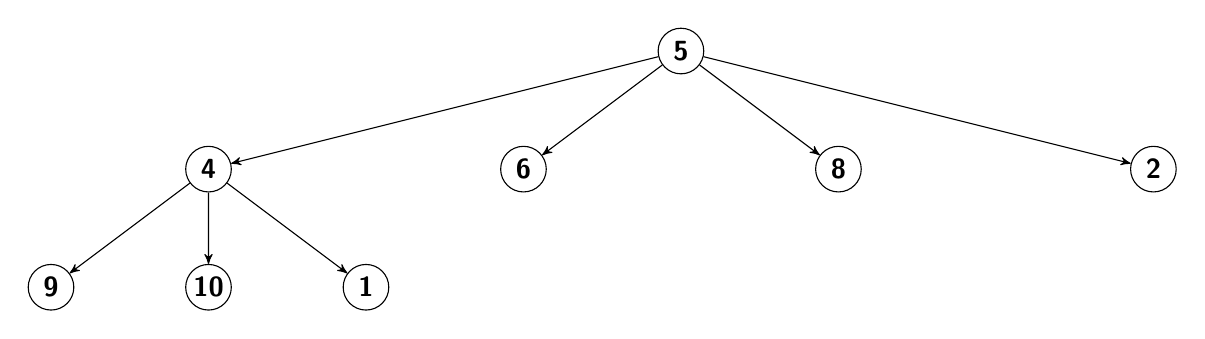
\begin{tikzpicture}[->,>=stealth',level/.style={sibling distance = 4cm/#1,
            level distance = 1.5cm}] 
            \node [arn_n] {5} % ROOT
            child{ node [arn_n] {4} 
                child{ node [arn_n] {9}}
                child{ node [arn_n] {10}}                            
                child{ node [arn_n] {1}}                            
            }
            child{ node [arn_n] {6}}
            child{ node [arn_n] {8}}
            child{ node [arn_n] {2}}
            ; 
        \end{tikzpicture}
        
        \item Looking at the tree you have drawn, how many leaves and nodes are present? 

        6 leaves, 8 nodes, 2 of which are internal.
        
        \item Examine your tree and find both the root and the node with the value 4. For both nodes, list the following attributes: depth, height of subtrees, number of siblings, number of children. 

        Root Node: \{ depth: 0, height of subtrees: [2, 1, 1, 1], number of siblings: 0, number of direct children: 4, descendants: 7 \}

        Node(4) \{ depth: 1, height of subtrees: [1, 1, 1, 0], number of siblings: 3, number of direct children: 3, descendants: 3 \}
        
        \item Insert 6 more random elements into your tree and relist any of the above attributes that have changed.

        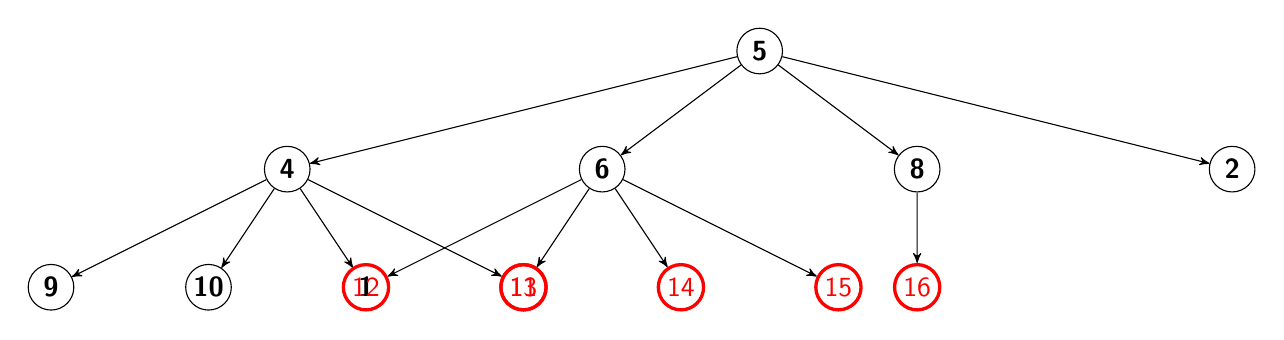
\begin{tikzpicture}[->,>=stealth',level/.style={sibling distance = 4cm/#1,
            level distance = 1.5cm}] 
            \node [arn_n] {5} % ROOT
            child{ node [arn_n] {4} 
                child{ node [arn_n] {9}}
                child{ node [arn_n] {10}}                            
                child{ node [arn_n] {1}}  
                child{ node [arn_r] {11}}                         
            }
            child{ node [arn_n] {6}
                child{ node [arn_r] {12}}
                child{ node [arn_r] {13}}
                child{ node [arn_r] {14}}
                child{ node [arn_r] {15}}
            }
            child{ node [arn_n] {8}
                child{ node [arn_r] {16}}
            }
            child{ node [arn_n] {2}}
            ; 
        \end{tikzpicture}

        Root Node: \{ depth: 0, height of subtrees: [2, 2, 2, 1], number of siblings: 0, number of direct children: 4, descendants: 13 \}

        Node(4) \{ depth: 1, height of subtrees: [1, 1, 1, 1], number of siblings: 3, number of direct children: 4, descendants: 4 \}
        
        \item Would the structure of the k-ary tree you've drawn change at all if the elements were inserted in sorted order? Explain why or why not.

        No. K-ary trees are not sorted trees.
    \end{enumerate}
    
    \section{Binary Trees}
    \begin{enumerate}
        \item Draw a binary tree after the insertion of the following elements in order: 
        
        \verb|[60, 40, 35, 75, 90, 1, 20, 100, 25, 70]|

        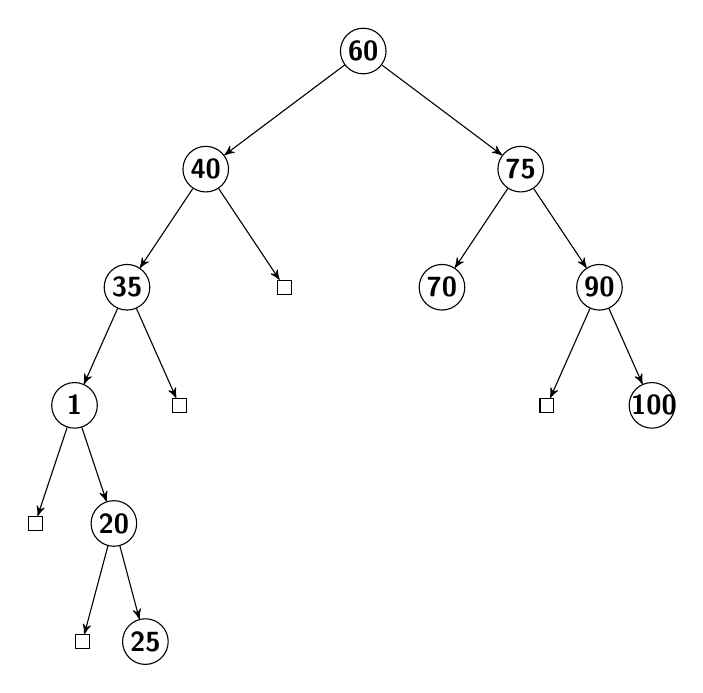
\begin{tikzpicture}[->,>=stealth',level/.style={sibling distance = 4cm/#1,
            level distance = 1.5cm}] 
            \node [arn_n] {60} % ROOT
            child{ node [arn_n] {40}
                child{ node [arn_n] {35}
                    child{ node [arn_n] {1}
                        child{ node [arn_x] {}}
                        child{ node [arn_n] {20}
                            child{ node [arn_x] {}}
                            child{ node [arn_n] {25}}
                        }
                    }
                    child{ node [arn_x] {}}
                }
                child{ node [arn_x] {}}
            }
            child{ node [arn_n] {75}
                child{ node [arn_n] {70}}
                child{ node [arn_n] {90}
                    child{ node [arn_x] {}}
                    child{ node [arn_n] {100}}
                }
            }
            ;
        \end{tikzpicture}
        
        \item Draw a binary tree after the insertion of the following elements in order: 
        
        \verb|[10, 20, 30, 40, 50, 60, 70, 80, 90, 100]|

        \begin{tikzpicture}[->,>=stealth',level/.style={sibling distance = 4cm/#1,
            level distance = 1.5cm}] 
            \node [arn_n] {10} % ROOT
            child{ node[arn_x] {}}
            child{ node [arn_n] {20}
                child{ node[arn_x] {}}
                child{ node [arn_n] {30}
                    child{ node[arn_x] {}}
                    child{ node [arn_n] {40}
                        child{ node[arn_x] {}}
                        child{ node [arn_n] {50}
                            child{ node[arn_x] {}}
                            child{ node [arn_n] {60}
                                child{ node[arn_x] {}}
                                child{ node [arn_n] {...}}
                            }
                        }
                    }
                }
            }
            ;
        \end{tikzpicture}
        
        \item Explain what differs in the above two trees. Specifically, address how many leaf nodes there are, the depth of the right, and leftmost nodes, and the height of both the left and right subtrees from the root node.

        The tree with elements inserted in sorted order only has one leaf, whereas the previous tree had 3. The sorted tree is also extremely imbalanced, with all elements going towards the right. 
        
        \item If a Binary Tree is complete, does that necessarily mean it is also full? Justify your answer with drawings of trees.

        No, the deepest layer of the tree could have a node that only possesses a single child.
        
        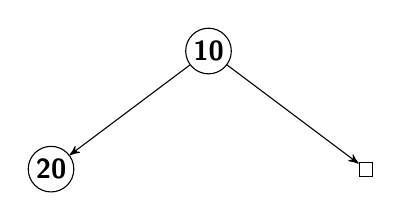
\begin{tikzpicture}[->,>=stealth',level/.style={sibling distance = 4cm/#1,
            level distance = 1.5cm}] 
            \node [arn_n] {10} % ROOT
            child{ node[arn_n] {20}}
            child{ node [arn_x] {}}
            ;
        \end{tikzpicture}

        Is complete, but not full.

    \end{enumerate}
    
    \section{Stacks and Queues}
    \begin{enumerate}
        \item Continuing from your previous \verb|LinkedList| solution, what changes would be required to convert this list into a generic queue? What about a stack?

        It would require modifying the API, simplifying the interface to allow fewer, operations.

        \item Is a linked list the best underlying structure to implement a queue with? Justify your answer. 

        Linked lists are a convenient underlying structure, but there is no true best when it comes to queues. So long as your implementation offers constant time operations and minimal space requirements.

        \item Implement both a queue, and a stack. Provide only the essential methods for both (Constructor, Destructor, Push, Pop, Peek), and use whatever underlying structure you would prefer.
    \end{enumerate}
    
    \label{r:lastpage}
    
    \end{document}
        
    